%Copyright 2014 Jean-Philippe Eisenbarth
%This program is free software: you can 
%redistribute it and/or modify it under the terms of the GNU General Public 
%License as published by the Free Software Foundation, either version 3 of the 
%License, or (at your option) any later version.
%This program is distributed in the hope that it will be useful,but WITHOUT ANY 
%WARRANTY; without even the implied warranty of MERCHANTABILITY or FITNESS FOR A 
%PARTICULAR PURPOSE. See the GNU General Public License for more details.
%You should have received a copy of the GNU General Public License along with 
%this program.  If not, see <http://www.gnu.org/licenses/>.

%Based on the code of Yiannis Lazarides
%http://tex.stackexchange.com/questions/42602/software-requirements-specification-with-latex
%http://tex.stackexchange.com/users/963/yiannis-lazarides
%Also based on the template of Karl E. Wiegers
%http://www.se.rit.edu/~emad/teaching/slides/srs_template_sep14.pdf
%http://karlwiegers.com
\documentclass{scrreprt}
\usepackage{listings}
\usepackage{underscore}
\usepackage[bookmarks=true]{hyperref}
\usepackage[utf8]{inputenc}
\usepackage[english]{babel}
\usepackage{pgfgantt}
\usepackage{CJKutf8}
\usepackage{graphicx}
\hypersetup{
    bookmarks=false,    % show bookmarks bar?
    pdftitle={Software Requirement Specification},    % title
    pdfauthor={Jean-Philippe Eisenbarth},                     % author
    pdfsubject={TeX and LaTeX},                        % subject of the document
    pdfkeywords={TeX, LaTeX, graphics, images}, % list of keywords
    colorlinks=true,       % false: boxed links; true: colored links
    linkcolor=blue,       % color of internal links
    citecolor=black,       % color of links to bibliography
    filecolor=black,        % color of file links
    urlcolor=purple,        % color of external links
    linktoc=page            % only page is linked
}%
\def\myversion{1.0 }
\date{}
%\title
\usepackage{hyperref}
\begin{document}

\begin{flushright}
    \rule{16cm}{5pt}\vskip1cm
    \begin{bfseries}
        \Huge{SOFTWARE REQUIREMENTS\\ SPECIFICATION}\\
        \vspace{1.9cm}
        for\\
        \vspace{1.0cm}
        $<$chatroom robot assistant$>$\\
        \vspace{1.0cm}
        \LARGE{Version \myversion approved}\\
        \vspace{1.0cm}
	\begin{CJK}{UTF8}{bkai}
        		 Prepared by :  \\
	   	1031408 劉彥呈\\
	   	1031452 何浩璘\\
	   	1033329 林仕翔\\
	   	1033336 尹法堯\\
        		1041459 梁澤洲\\
        \vspace{1.0cm}
        $<$開放平台軟體 第15組$>$\\
        \vspace{1.0cm}
        \today\\
	\end{CJK}
    \end{bfseries}
\end{flushright}

\tableofcontents


\chapter*{Revision History}

\begin{CJK}{UTF8}{bkai}
	\begin{center}
    		\begin{tabular}{|c|c|c|c|c|}
        		\hline
	    	學號 & Name & Date & Reason For Changes & Version\\
        		\hline
	   	1031408 & 劉彥呈 & 5/19 & 顯示時間 & 1\\
        		\hline
	    	1033336 & 尹法堯 & 5/19 & Client進入訊息 & 2\\
        		\hline
		1031408 & 劉彥呈 & 5/20 & Client離開訊息 & 3\\
        		\hline
		1033336 & 尹法堯 & 5/20 & 區分相同的name & 4\\
        		\hline
		1033336 & 尹法堯 & 6/14 & 完成資料庫所有功能和Server新增帳號 & 5\\
		\hline
		1031408 & 劉彥呈 & 6/14 & 完成資料庫與介面的互動 & 5\\
        		\hline
		1031408 & 劉彥呈 & 6/17 & 顯示再現人數 & 7\\
        		\hline
		1033336 & 尹法堯 & 6/18 &  Server刪除帳號& 8\\
        		\hline
		1031408 & 劉彥呈 & 6/19 & Server踢除Client & 9\\
        		\hline
		1031452 & 何浩璘 & 6/19 & Bot加入以及weather-api的使用 & 10\\
        		\hline
		1031408 & 劉彥呈 & 6/19 & 更換介面的顏色 & 11\\
        		\hline
		1031452 & 何浩璘 & 6/23 & Bot增加匯率轉換-api和顯示日期區域時間 & 12\\
        		\hline
    		\end{tabular}
	\end{center}


\chapter{Introduction}

\section{Purpose}
該文件提供cahtroom robot assistant Version12的相關說明,包含改產品的開發理念、最終
成果,產品的提供對象及適用範圍,系統的程式碼架構,不同物件之間的上下關係,程式運行環境以及產品特色

\section{Document Conventions}
$<$Describe any standards or typographical conventions that were followed when 
writing this SRS, such as fonts or highlighting that have special significance.  
For example, state whether priorities  for higher-level requirements are assumed 
to be inherited by detailed requirements, or whether every requirement statement 
is to have its own priority.$>$

\section{Intended Audience and Reading Suggestions}
本文件適合以下職位的人員觀看,部分內容須有程式邏輯相關知識: \\
(1)專案經理:專案經理可以根據該文檔瞭解預期產品的功能,以此進行系統設計。 \\
(2)設計員:對需求進行分析,並設計出系統,包括資料庫的設計。 \\
(3)程式師:瞭解系統功能,對後續更新版本或產品維護提供程式架構。 \\
(4)測試員:根據本文檔對軟體產品進行功能性測試和非功能性測試。 \\
(5)銷售人員:瞭解預期產品的功能和性能。 \\
(6)用戶:瞭解預期產品的功能和性能,與分析人員對整個需求進行討論和協商。 \\


\section{Project Scope}
該產品的開發理念為節省使用者在聊天室與夥伴聊天時,為查詢生活中的小資訊而必須頻繁切換應用程式的時間
,希望使用者可以在與夥伴聊天時,在時間上有很好的使用者體驗,或者討論單日行的旅遊,或者與分隔兩地的朋友聊天時,
可以方便的查詢當地天氣相關資訊以提供聊天話題。

\section{References}
1. https://pypi.org/project/weather-api/ \\
2. https://pypi.org/project/currency.converter/ \\
3. http://pyqt.sourceforge.net/Docs/PyQt5/ \\



\chapter{Overall Description}

\section{Product Perspective}
$<$Describe the context and origin of the product being specified in this SRS.  
For example, state whether this product is a follow-on member of a product 
family, a replacement for certain existing systems, or a new, self-contained 
product. If the SRS defines a component of a larger system, relate the 
requirements of the larger system to the functionality of this software and 
identify interfaces between the two. A simple diagram that shows the major 
components of the overall system, subsystem interconnections, and external 
interfaces can be helpful.$>$

\section{Product Functions}
$<$Summarize the major functions the product must perform or must let the user 
perform. Details will be provided in Section 3, so only a high level summary 
(such as a bullet list) is needed here. Organize the functions to make them 
understandable to any reader of the SRS. A picture of the major groups of 
related requirements and how they relate, such as a top level data flow diagram 
or object class diagram, is often effective.$>$

\section{User Classes and Characteristics}
$<$Identify the various user classes that you anticipate will use this product.  
User classes may be differentiated based on frequency of use, subset of product 
functions used, technical expertise, security or privilege levels, educational 
level, or experience. Describe the pertinent characteristics of each user class.  
Certain requirements may pertain only to certain user classes. Distinguish the 
most important user classes for this product from those who are less important 
to satisfy.$>$

\section{Operating Environment}
1. OS: Window7 以上版本 (未在其他作業系統測試過) \\
2. 開發語言: python3 \\
3. 使用python api: weather-api, currency_converter \\
4. 其他python開發套件: socket, threading, os, sys, time, PyQt5 \\
5. 資料庫: mongoDB

\section{Design and Implementation Constraints}
$<$Describe any items or issues that will limit the options available to the 
developers. These might include: corporate or regulatory policies; hardware 
limitations (timing requirements, memory requirements); interfaces to other 
applications; specific technologies, tools, and databases to be used; parallel 
operations; language requirements; communications protocols; security 
considerations; design conventions or programming standards (for example, if the 
customer’s organization will be responsible for maintaining the delivered 
software).$>$

\section{User Documentation}
$<$List the user documentation components (such as user manuals, on-line help, 
and tutorials) that will be delivered along with the software. Identify any 
known user documentation delivery formats or standards.$>$

\section{Assumptions and Dependencies}

$<$List any assumed factors (as opposed to known facts) that could affect the 
requirements stated in the SRS. These could include third-party or commercial 
components that you plan to use, issues around the development or operating 
environment, or constraints. The project could be affected if these assumptions 
are incorrect, are not shared, or change. Also identify any dependencies the 
project has on external factors, such as software components that you intend to 
reuse from another project, unless they are already documented elsewhere (for 
example, in the vision and scope document or the project plan).$>$



\begin{ganttchart}[%Specs
     y unit title=0.5cm,
     y unit chart=0.6cm,
     vgrid,hgrid,
     title height=1,
%     title/.style={fill=none},
     title label font=\bfseries\normalsize,
     bar/.style={fill=blue},
     bar height=0.5,
%   progress label text={},
     group right shift=0,
     group top shift=0.5,
     group height=.3,
     group peaks width={0.2},
     inline]{1}{24}
    %labels
    \gantttitle{Title}{24}\\  % title 1
	\gantttitle{1}{2}                      % title 3
	\gantttitle{2}{2}
	\gantttitle{3}{2}
    	\gantttitle{4}{2}
	\gantttitle{5}{2}
	\gantttitle{6}{2}
	\gantttitle{7}{2}
	\gantttitle{8}{2}
	\gantttitle{9}{2}
	\gantttitle{10}{2}
	\gantttitle{11}{2}
	\gantttitle{12}{2}\\
    % Setting group if any
    \ganttgroup[inline=false]{A}{1}{12}\\ 
    \ganttbar[inline=false, bar progress label node/.append style={below left= 10pt and 7pt}]{\small a}{3}{4}\\ 
      \ganttmilestone[inline=false]{\small b}{6}\\ 
\end{ganttchart}


\chapter{External Interface Requirements}

\section{User Interfaces}
\begin{figure}[h]
\begin{center}
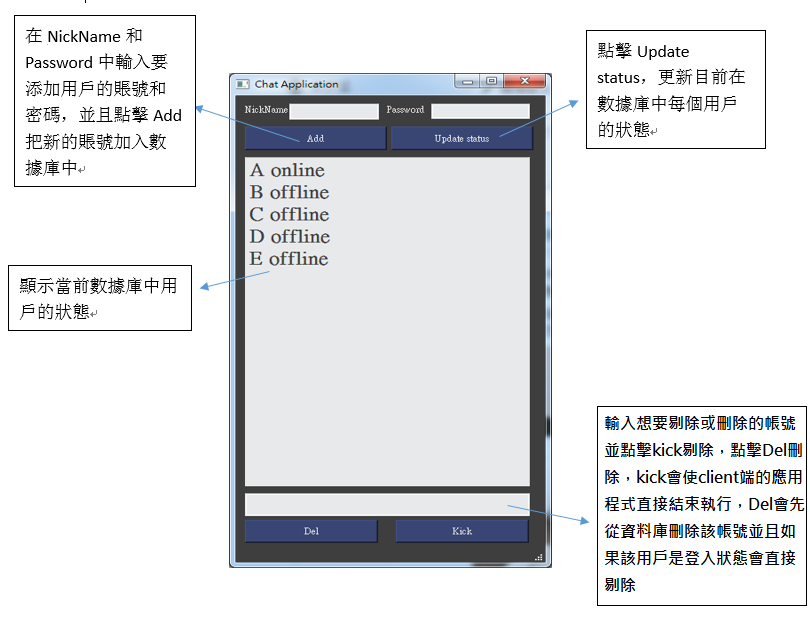
\includegraphics[width=15cm]{interface1.png}
+\end{center}
\caption{sever interface}
\label{fig:2}
\end{figure}

\begin{figure}[h]
\begin{center}
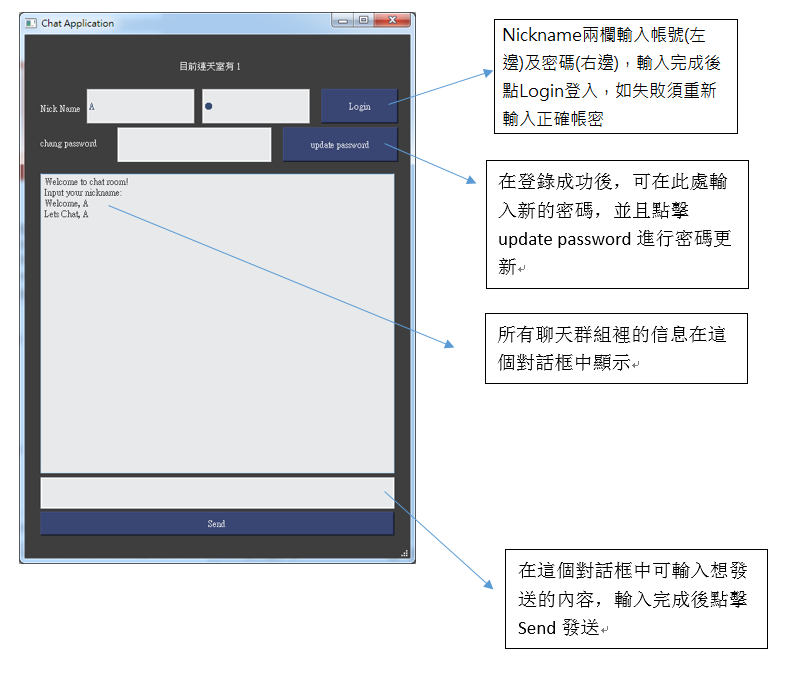
\includegraphics[width=15cm]{interface2.png}
\end{center}
\caption{client interface}
\label{fig:3}
\end{figure}

\section{Hardware Interfaces}
$<$Describe the logical and physical characteristics of each interface between 
the software product and the hardware components of the system. This may include 
the supported device types, the nature of the data and control interactions 
between the software and the hardware, and communication protocols to be 
used.$>$

\section{Software Interfaces}
一、 資料庫 \\
(1) mongoDB 3.6 : 用於管理帳號密碼以及狀態資訊 \\
二、python 套件 \\
(1) socket : 用於處理server與client之間的訊息傳遞 \\
(2) threading : 用與處理接收訊息、傳遞訊息、GUI之間的線程管理 \\
(3) os : 用於強制讓程式結束運作\\
(4) time : 用於顯示發送或接收訊息時,當下的時間資訊\\
(5) PyQt5 5.10.1 : 用於呈現server與client的UI介面、按鈕事件控制\\
(6) pymongo 3.6.4 : python用於控制mongoDB的函示庫\\
(7) weather-api 1.0.4 : 用於取得某地的天氣資訊,輸入為地區名稱,輸出會當地溫度、天氣狀況、濕度等資訊\\
(8) CurrencyConverter 0.13.5 : 用於轉換兩個不同的貨幣,輸入為金額、原始貨幣、轉換後貨幣,輸出為轉換後貨幣的金額 \\

\section{Communications Interfaces}
$<$Describe the requirements associated with any communications functions 
required by this product, including e-mail, web browser, network server 
communications protocols, electronic forms, and so on. Define any pertinent 
message formatting. Identify any communication standards that will be used, such 
as FTP or HTTP. Specify any communication security or encryption issues, data 
transfer rates, and synchronization mechanisms.$>$


\chapter{System Features}
$<$This template illustrates organizing the functional requirements for the 
product by system features, the major services provided by the product. You may 
prefer to organize this section by use case, mode of operation, user class, 
object class, functional hierarchy, or combinations of these, whatever makes the 
most logical sense for your product.$>$

\section{System Feature 1}
$<$Don’t really say “System Feature 1.” State the feature name in just a few 
words.$>$

\subsection{Description and Priority}
$<$Provide a short description of the feature and indicate whether it is of 
High, Medium, or Low priority. You could also include specific priority 
component ratings, such as benefit, penalty, cost, and risk (each rated on a 
relative scale from a low of 1 to a high of 9).$>$

\subsection{Stimulus/Response Sequences}
$<$List the sequences of user actions and system responses that stimulate the 
behavior defined for this feature. These will correspond to the dialog elements 
associated with use cases.$>$

\subsection{Functional Requirements}
$<$Itemize the detailed functional requirements associated with this feature.  
These are the software capabilities that must be present in order for the user 
to carry out the services provided by the feature, or to execute the use case.  
Include how the product should respond to anticipated error conditions or 
invalid inputs. Requirements should be concise, complete, unambiguous, 
verifiable, and necessary. Use “TBD” as a placeholder to indicate when necessary 
information is not yet available.$>$

$<$Each requirement should be uniquely identified with a sequence number or a 
meaningful tag of some kind.$>$

REQ-1:	REQ-2:

\section{System Feature 2 (and so on)}


\chapter{Other Nonfunctional Requirements}

\section{Performance Requirements}
$<$If there are performance requirements for the product under various 
circumstances, state them here and explain their rationale, to help the 
developers understand the intent and make suitable design choices. Specify the 
timing relationships for real time systems. Make such requirements as specific 
as possible. You may need to state performance requirements for individual 
functional requirements or features.$>$

\section{Safety Requirements}
$<$Specify those requirements that are concerned with possible loss, damage, or 
harm that could result from the use of the product. Define any safeguards or 
actions that must be taken, as well as actions that must be prevented. Refer to 
any external policies or regulations that state safety issues that affect the 
product’s design or use. Define any safety certifications that must be 
satisfied.$>$

\section{Security Requirements}
$<$Specify any requirements regarding security or privacy issues surrounding use 
of the product or protection of the data used or created by the product. Define 
any user identity authentication requirements. Refer to any external policies or 
regulations containing security issues that affect the product. Define any 
security or privacy certifications that must be satisfied.$>$

\section{Software Quality Attributes}
$<$Specify any additional quality characteristics for the product that will be 
important to either the customers or the developers. Some to consider are: 
adaptability, availability, correctness, flexibility, interoperability, 
maintainability, portability, reliability, reusability, robustness, testability, 
and usability. Write these to be specific, quantitative, and verifiable when 
possible. At the least, clarify the relative preferences for various attributes, 
such as ease of use over ease of learning.$>$

\section{Business Rules}
$<$List any operating principles about the product, such as which individuals or 
roles can perform which functions under specific circumstances. These are not 
functional requirements in themselves, but they may imply certain functional 
requirements to enforce the rules.$>$


\chapter{Other Requirements}
$<$Define any other requirements not covered elsewhere in the SRS. This might 
include database requirements, internationalization requirements, legal 
requirements, reuse objectives for the project, and so on. Add any new sections 
that are pertinent to the project.$>$

\section{Appendix A: Glossary}
%see https://en.wikibooks.org/wiki/LaTeX/Glossary
$<$Define all the terms necessary to properly interpret the SRS, including 
acronyms and abbreviations. You may wish to build a separate glossary that spans 
multiple projects or the entire organization, and just include terms specific to 
a single project in each SRS.$>$

\section{Appendix B: Analysis Models}
$<$Optionally, include any pertinent analysis models, such as data flow 
diagrams, class diagrams, state-transition diagrams, or entity-relationship 
diagrams.$>$

\section{Appendix C: To Be Determined List}
$<$Collect a numbered list of the TBD (to be determined) references that remain 
in the SRS so they can be tracked to closure.$>$

\end{CJK}
\end{document}
